\documentclass[aspectratio=169,11pt]{beamer}
\usetheme[progressbar=frametitle,numbering=fraction]{metropolis}
\usepackage{booktabs}
\usepackage{qrcode}
\usepackage{tikz}
\usetikzlibrary{positioning,arrows.meta}
\definecolor{borg}{HTML}{1B6E5A}
\setbeamercolor{progress bar}{fg=borg}
\setbeamercolor{frametitle}{bg=borg!85!black}
\setbeamercolor{alerted text}{fg=borg}
\newcommand{\footage}[1]{\begin{center}\fbox{\parbox{0.8\linewidth}{\centering\vspace{2cm}\textit{footage: #1}\vspace{2cm}}}\end{center}}

\title{Borg: Vulkan from vkcube Down to the Gates}
\subtitle{Vulkanised 2027 Video Vault}
\author{Andreas Wendleder}
\date{}

\begin{document}

% 0. Cold open
\begin{frame}[plain]
  \footage{unmodified vkcube on the ULX3S over HDMI, 30 s, no words}
\end{frame}

\maketitle

% 1. What Borg is
\section{What Borg is}

\begin{frame}{An open GPU you can read end to end}
  \begin{itemize}
    \item The GPU: about 12,300 lines of Chisel. FP32 shader core running 2x2 quads, tile-based rasterizer,
      texture unit, MSAA, compute.
    \item The system around it: Hutt, a small RISC-V CPU.
    \item The driver: borgvk, a native Mesa Vulkan driver in Rust, with its own shader compiler, borgc.
    \item One source, three targets: ULX3S (ECP5), Nexys Video (Artix-7), GF180 ASIC.
    \item Everything open source.
  \end{itemize}
\end{frame}

\begin{frame}{One driver, three back ends}
  \centering
  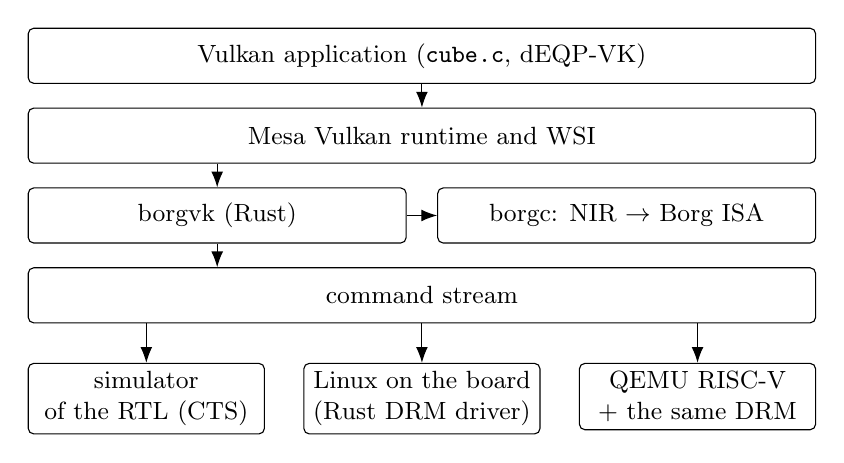
\begin{tikzpicture}[box/.style={draw, rounded corners=2pt, align=center, font=\small, minimum height=7mm,
      inner sep=3pt}, arr/.style={-{Latex[length=2mm]}}]
    \node[box, minimum width=10cm] (app) {Vulkan application (\texttt{cube.c}, dEQP-VK)};
    \node[box, minimum width=10cm, below=3mm of app] (rt) {Mesa Vulkan runtime and WSI};
    \node[box, minimum width=4.8cm, below=3mm of rt.south west, anchor=north west] (vk) {borgvk (Rust)};
    \node[box, minimum width=4.8cm, below=3mm of rt.south east, anchor=north east] (cc) {borgc: NIR $\to$ Borg ISA};
    \node[box, minimum width=10cm, below=3mm of vk.south west, anchor=north west] (pk) {command stream};
    \node[box, below=5mm of pk.south west, anchor=north west, minimum width=3cm] (sim) {simulator\\of the RTL (CTS)};
    \node[box, below=5mm of pk.south, minimum width=3cm] (lin) {Linux on the board\\(Rust DRM driver)};
    \node[box, below=5mm of pk.south east, anchor=north east, minimum width=3cm] (qemu) {QEMU RISC-V\\+ the same DRM};
    \draw[arr] (app) -- (rt); \draw[arr] (rt.south -| vk) -- (vk); \draw[arr] (vk) -- (cc);
    \draw[arr] (vk.south) -- (vk.south |- pk.north);
    \draw[arr] (pk.south -| sim) -- (sim); \draw[arr] (pk) -- (lin); \draw[arr] (pk.south -| qemu) -- (qemu);
  \end{tikzpicture}
\end{frame}

% 2. What Vulkan 1.0 asks of hardware
\section{What Vulkan 1.0 asks of hardware}

\begin{frame}{Requirements that became hardware}
  \centering\small
  \begin{tabular}{ll}
    \toprule
    Vulkan 1.0 requirement & Borg mechanism \\
    \midrule
    Compute on every graphics queue & workgroup dispatch, barrier, atomics \\
    Derivatives, implicit LOD & 2x2 quad on four lanes \\
    Sampled images, samplers & descriptor-table texture unit, 51 formats, mipmaps \\
    Colour attachment formats & raw attachments, blending by read-back \\
    Depth, stencil, scissor, blend & fixed function in the tile pipeline \\
    Occlusion queries & exact passing-sample counts \\
    4x MSAA & multiple passes per tile \\
    Vertex input, topologies & hardware draw front end \\
    \bottomrule
  \end{tabular}
\end{frame}

\begin{frame}{A graphics queue implies compute}
  \begin{itemize}
    \item Every queue family with graphics must also do compute.
    \item Workgroups run on the same shader core: barrier, atomics, shared memory.
    \item It matters far beyond compute apps: the CTS runs \texttt{glsl.builtin.precision} as compute
      dispatches, so this path gates thousands of shader tests.
  \end{itemize}
\end{frame}

\begin{frame}{Derivatives need quads}
  \begin{itemize}
    \item \texttt{dFdx}, \texttt{dFdy}: differences between neighbouring pixels.
    \item So the fragment core runs a 2x2 quad on four lanes; implicit LOD uses the same quad.
    \item A one-lane core is smaller and returns zero derivatives.
  \end{itemize}
\end{frame}

\begin{frame}{Descriptors become hardware tables}
  \begin{itemize}
    \item The texture unit reads Vulkan's image and sampler state from tables in memory, which the
      driver fills directly.
    \item 51 formats, mipmaps, every address mode and border colour, gather, compare, offsets.
    \item Render targets use the same tiled layout: rendering to a texture needs no copy.
  \end{itemize}
\end{frame}

\begin{frame}{The draw front end}
  \begin{itemize}
    \item One register write renders a whole draw.
    \item Primitive assembly: lists, strips, fans, indices, restart, instancing.
    \item One vertex shader run per triangle; varyings out and back by two instructions.
    \item Homogeneous 2D setup: no clipping needed, vertices behind the eye are exact.
  \end{itemize}
\end{frame}

% 3. Driver and compiler
\section{A driver and compiler for 32 registers}

\begin{frame}{borgvk and borgc}
  \begin{itemize}
    \item Mesa's Vulkan runtime for objects, synchronization and WSI; borgvk in Rust,
      about 12,000 lines.
    \item borgc takes NIR after Mesa's lowering; one instruction selector for graphics and compute.
    \item 32 registers per lane; the ISA moves to a RISC-V subset plus GPU instructions.
    \item Refuse instead of guess: a refused pipeline is an honest CTS failure, a miscompiled one
      can pass by luck.
  \end{itemize}
\end{frame}

\begin{frame}[fragile]{One source of truth for the ISA}
  \small
\begin{verbatim}
add      rd rs1 rs2     31..25=0 14..12=0 6..2=0x0C 1..0=3
fmadd.s  rd rs1 rs2 rs3 rm 26..25=0 6..2=0x10 1..0=3
texd     rd rs1 rs2 rs3 26..25=0 14..12=0 6..2=0x0A 1..0=3
sout.v2  rs2 index      31..25=0 14..12=0 6..2=0x16 1..0=3
\end{verbatim}
  \normalsize
  \begin{itemize}
    \item The format of RISC-V's \texttt{riscv-opcodes}.
    \item The hardware decoder, the C header and the compiler's encoder are generated from it.
    \item A corpus of recorded shaders checks every compiler change.
  \end{itemize}
\end{frame}

\begin{frame}{Per-draw work out of the fragment shader}
  \begin{itemize}
    \item What a fragment shader computes from push constants alone is the same for every pixel.
    \item \texttt{nir\_opt\_preamble} finds it; the vertex shader runs it once per triangle and
      passes it on as flat varyings.
    \item Other GPUs run such a preamble once per draw; Borg has no unit for that, so the vertex
      shader is the cheapest place.
  \end{itemize}
  \centering\small
  \begin{tabular}{lrr}
    \toprule
    Instructions & fragment (per pixel) & vertex (per triangle) \\
    \midrule
    before & 320 & 87 \\
    after  & 133 & 281 \\
    \bottomrule
  \end{tabular}
\end{frame}

% 4. CTS against RTL
\section{Running the CTS against the RTL}

\begin{frame}{The direct simulator}
  \begin{itemize}
    \item The GPU's RTL, without CPU, compiled to native code with CIRCT's arcilator.
    \item Driven by the same command stream as the hardware; the CTS sees an ordinary Vulkan device.
    \item About 120,000 cycles per second per instance, many instances in parallel, sharded on CI.
  \end{itemize}
\end{frame}

\begin{frame}{Live: CTS cases on the simulator}
  \footage{terminal: \texttt{scripts/cts\_par.sh} on a handful of cases, results coming in}
\end{frame}

\begin{frame}{Throughput decides what you can test}
  \begin{itemize}
    \item Compute precision cases use one invocation per workgroup: three of four quad lanes idle.
      Packing four workgroups into one quad: \texttt{atan2} vec4 from over 40 minutes to about two.
    \item Large render passes split into strips across simulators, per-draw work hoisted:
      a pipeline barrier case from a 5.5 h timeout to a pass in under 2 h.
  \end{itemize}
\end{frame}

\begin{frame}{Bugs found before silicon}
  \begin{itemize}
    \item \texttt{textureGather} at cube corners returned one subtap instead of the average.
    \item Integer bits copied through a float move were flushed when they looked like denormals.
    \item Branch targets in fragment programs landed one word early.
    \item A constant was built after the instructions that read it.
    \item A simulator read gave up early, so slow cases passed with a half-drawn image.
  \end{itemize}
\end{frame}

\begin{frame}{Where it stands}
  \centering
  \textit{table and chart from a fresh full CTS run (to be added)}
\end{frame}

% 5. Lessons
\section{Lessons and what is next}

\begin{frame}{Lessons for a new implementation}
  \begin{itemize}
    \item Bring up the \texttt{api} group first, and compute early.
    \item Make the simulator fast before chasing failures.
    \item Refuse what the compiler cannot do.
    \item Keep one source of truth for the ISA.
    \item Distrust a pass that comes too fast.
    \item Record what the driver sends; check refactorings against it in minutes.
  \end{itemize}
\end{frame}

\begin{frame}{Next}
  \begin{itemize}
    \item The full Vulkan 1.0 must-pass list.
    \item The Nexys Video with Linux and DDR3.
    \item A tapeout.
  \end{itemize}
\end{frame}

\begin{frame}{Thank you}
  \centering
  \begin{tabular}{cc}
    \qrcode[height=3cm]{https://github.com/gonsolo/Borg} & \qrcode[height=3cm]{https://gonsolo.github.io/Borg/} \\[2mm]
    \small github.com/gonsolo/Borg & \small gonsolo.github.io/Borg \\
  \end{tabular}
\end{frame}

\end{document}
